\chapter{Specifications} \label{specifications}

\section{Overview}

The AHB-Lite PLIC IP core is a fully parameterised Platform-Level Interrupt
Controller, featuring a single AHB-Lite Slave interface and support for a user-defined number of both Interrupt Sources and Targets.

The purpose of the PLIC core is to connect multiple interrupt sources to
one or more interrupt targets. The core supports a programmable number
of simultaneous pending interrupt requests per source and individual routing of those interrupt requests to each target.

Per the \href{https://github.com/riscv/riscv-isa-manual/blob/master/release/riscv-privileged-v1.9.1.pdf}{RISC-V Privileged Architecture Instruction Set specification (v1.9.1)}, the core performs full interrupt prioritisation of each interrupt source; each may be assigned a separate priority and enabled per target via a matrix of interrupt enable bits. Further, an optional priority threshold per target may be defined to mask lower priority interrupts.

To reduce latency, the PLIC core presents all asserted interrupts to the target in priority order, queuing them so that a software interrupt handler can service all pending interrupts without the need to restore the interrupted context.

For illustration, a simplified example system using the PLIC core is shown below:

\begin{figure}[!htb]
	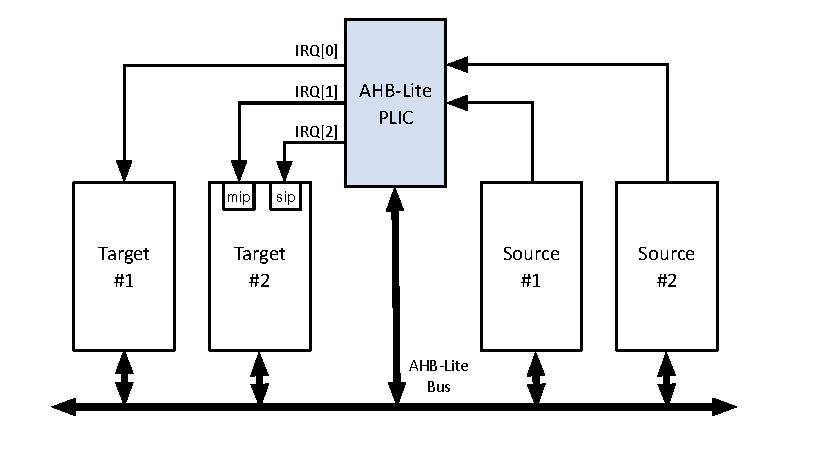
\includegraphics{assets/img/plic-system}
	\caption{PLIC System Diagram}
	\label{fig:SYSDIAG}
\end{figure}

\section{PLIC Operation}

The PLIC connects global \emph{interrupt sources}, which are usually
I/O devices, to \emph{interrupt targets}, which are usually \emph{hart
  contexts}.  The PLIC contains multiple \emph{interrupt gateways}, one
per interrupt source, together with a \emph{PLIC core} that performs
interrupt prioritization and routing.  Global interrupts are sent from
their source to an \emph{interrupt gateway} that processes the
interrupt signal from each source and sends a single \emph{interrupt
  request} to the PLIC core, which latches these in the core interrupt
pending bits (IP).  Each interrupt source is assigned a separate
priority.  The PLIC core contains a matrix of interrupt enable (IE)
bits to select the interrupts that are enabled for each target.  The
PLIC core forwards an \emph{interrupt notification} to one or more
targets if the targets have any pending interrupts enabled, and the
priority of the pending interrupts exceeds a per-target threshold.
When the target takes the external interrupt, it sends an \emph{
  interrupt claim} request to retrieve the identifier of the
highest-priority global interrupt source pending for that target from
the PLIC core, which then clears the corresponding interrupt source
pending bit.  After the target has serviced the interrupt, it sends
the associated interrupt gateway an \emph{interrupt completion} message
and the interrupt gateway can now forward another interrupt request
for the same source to the PLIC.  The rest of this chapter describes
each of these components in detail, though many details are
necessarily platform specific. 

\begin{figure}[tb]
\centering
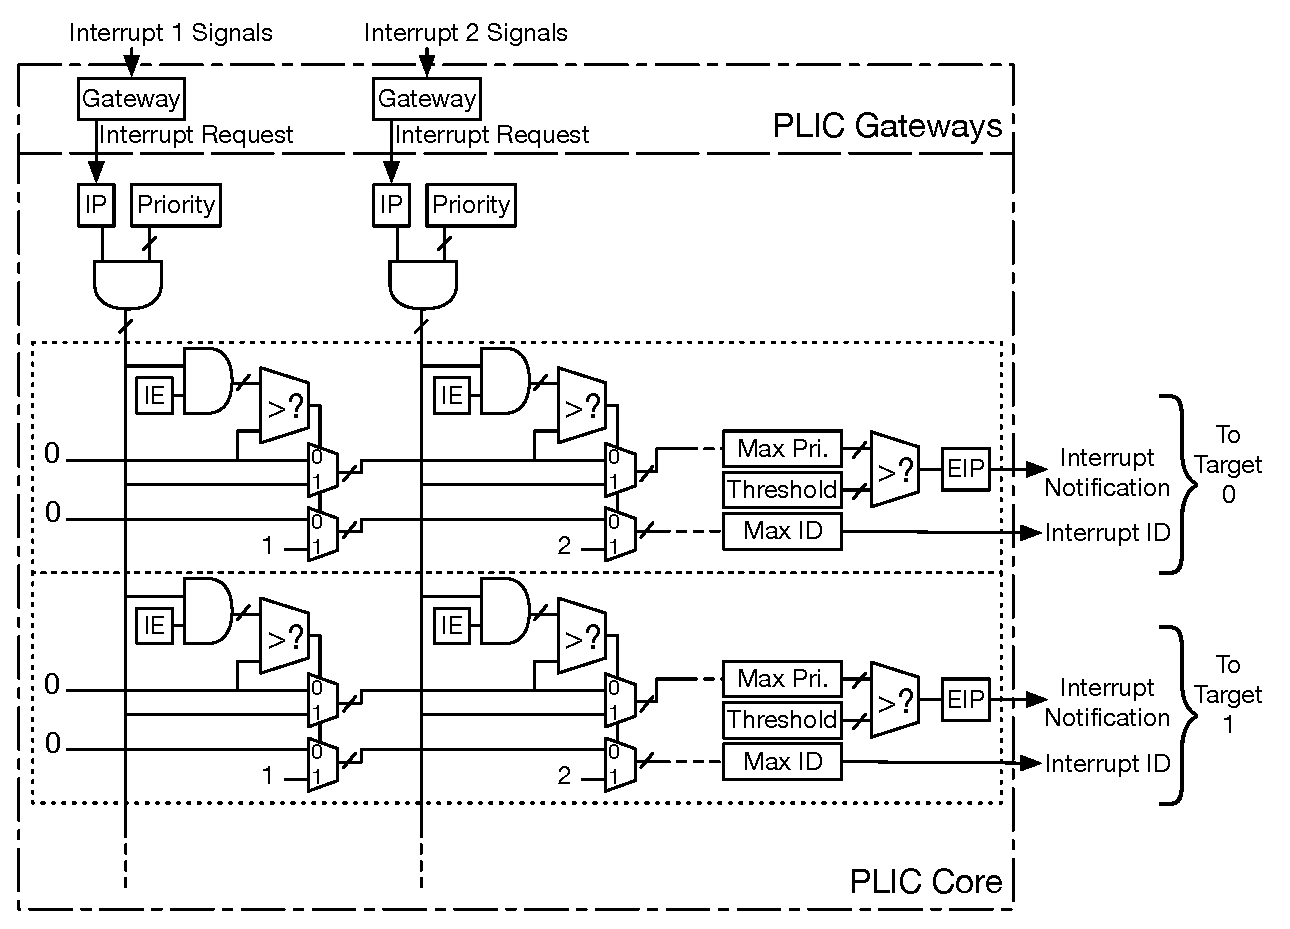
\includegraphics[width=\textwidth]{assets/img/PLIC-block-diagram}
\caption{Platform-Level Interrupt Controller (PLIC) conceptual block diagram.}
\label{fig:plic-block-diagram}
\end{figure}

\ifdefined\MARKDOWN
The figure above
\else
Figure~\ref{fig:plic-block-diagram} 
\fi
 provides an overview of PLIC operation, showing the first two of potentially many interrupt sources, and the first two of potentially many interrupt targets. 

\section{Interrupt Handling Handshake}

\subsection{Overview}

\ifdefined\MARKDOWN
The following figure
\else
Figure \ref{fig:HANDSHAKE} 
\fi
shows the logical flow of the handshake and the following sections describe the stages referenced: Interrupt Request, Interrupt Notification, Interrupt Claim Response, Processing the Interrupt and Interrupt Completion.

\begin{figure}[!htb]

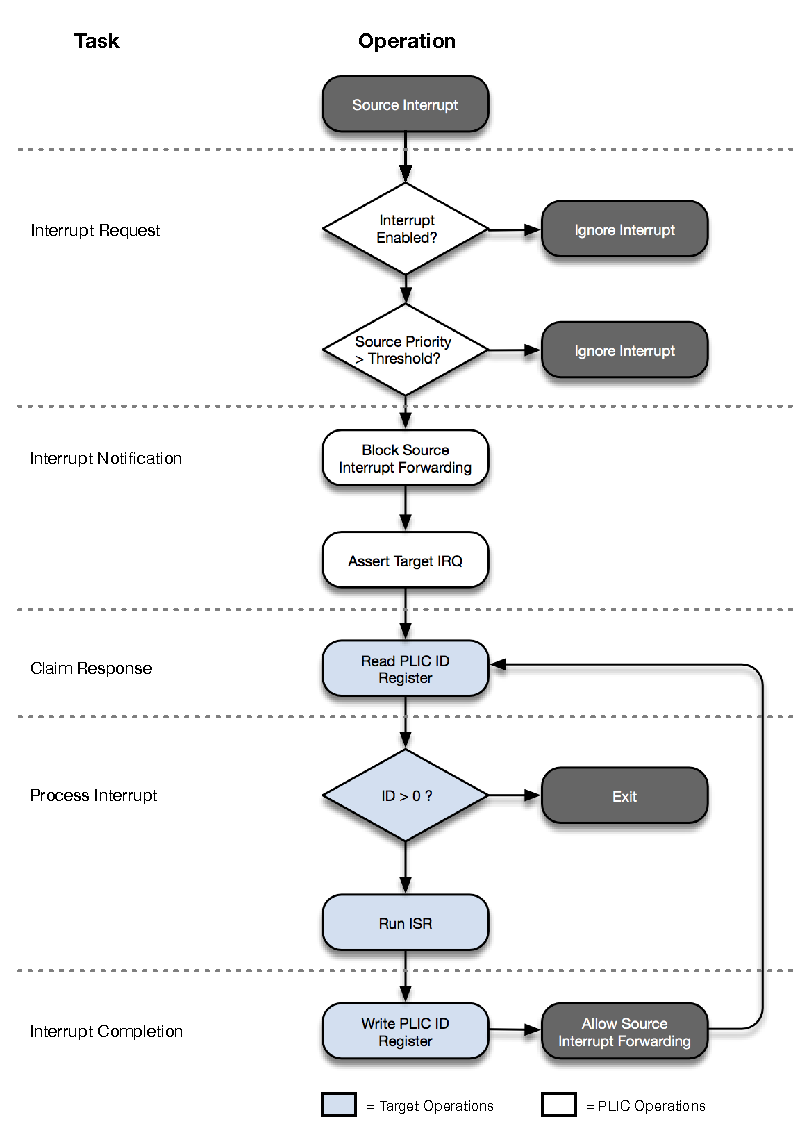
\includegraphics{assets/img/plic-handshake}
\caption{Interrupt Handling Handshake}
\label{fig:HANDSHAKE}
\end{figure}

Prior to operation, the PLIC system must be defined and configured as follows:

\begin{itemize}
	\item
		Each source must be assigned an Interrupt Identifier (\texttt{ID}) - a unique unsigned integer. This identifier will determine interrupt priority when 2 or more interrupts with the same priority level are asserted; The \emph{lower} the \texttt{ID} assigned to the source, the \emph{greater} the interrupt priority
	\item
		A matrix of Interrupt Enable vectors - one IE register per target - must be set to determine which target processes the interrupts from which source.
	\item
		Each Interrupt Source attached to the PLIC assigned a Priority Level - an unsigned integer value - that determines the relative priority of the interrupt source. Larger values have higher priority.
	\item
		Optionally, a Priority Threshold per target set to mask lower priority interrupts such that interrupts will only be presented to a target if the assigned Priority Level is greater than the Priority Threshold.
\end{itemize}

\subsection{Interrupt Request Stage}

A source asserts an interrupt request to the PLIC. The PLIC validates
the request by first checking if an interrupt enable bit is set for each
target and if the priority of the interrupt source exceeds any defined
Interrupt Priority Threshold. If these conditions do not hold, the
Interrupt Request is deemed invalid and stalled pending updates to the interrupt enable and/or priority threshold bits. 

The PLIC also determines if a previous interrupt request has been made by the same source.
If an interrupt is defined as level triggered and has already been asserted but not yet serviced, the request is ignored.
If an interrupt is defined as edge triggered and has already been asserted but not yet serviced, the request is queued by incrementing its Interrupt Pending counter.
The depth of this counter is parameterised.

If the request is deemed valid the request is forwarded to the
appropriate target. In the case of queued edge-triggered requests, the
interrupt pending counter is decremented by one immediately upon claim of the interrupt by the target.

\subsection{Interrupt Notification Stage}

A target is notified of an interrupt request by asserting the IRQ output for that target.
The PLIC blocks forwarding any further requests from the interrupt source until the current request is serviced.

On each clock cycle the ID register is loaded with the unique identifier of the highest priority interrupt to be processed.
This ensures that the Interrupt Service Routine always reads the highest pending interrupt request.

\subsection{Claim Response Stage} \label{sec:claim-response}

A target makes an interrupt claim response by reading its ID register.
This notifies the target of the interrupt source to service.
If the target has other interrupt sources pending, the IRQ output remains asserted, otherwise the IRQ output is negated.

\subsection{Interrupt Handler Stage}

If the ID read is greater than zero, the target services the identified interrupt source.
If the ID read is zero, this indicates no outstanding pending interrupts remain and the handler may terminate.

\subsection{Interrupt Completion Stage}

Once an interrupt has been serviced, completion is signalled to the PLIC by writing to the ID register.
The act of writing to the register is the completion notification; the value written is irrelevant.

On receiving the completion notification the PLIC will again allow interrupts to be forwarded from the corresponding source.

The Interrupt Handler may then exit, however it is possible a new
interrupt request may have been asserted while the handler was running.
To reduce latency the handler may instead determine if a new interrupt
has been received and if so again claim the interrupt (See earlier). In this
way the interrupt handler can service all interrupts without the need to
restore the interrupted context.


